\documentclass[conference]{IEEEtran}
\usepackage[utf8]{inputenc}
\usepackage[T1]{fontenc}
\IfFileExists{brazilian.ldf}{\usepackage[brazilian]{babel}}{}
\usepackage{graphicx}
\usepackage{booktabs}
\usepackage{amsmath}
\usepackage{url}
\usepackage{cite}

\begin{document}

\title{EcoSort: Assistente Multimodal de Descarte de Res\'iduos com Vis\~ao Computacional, PLN e Agente de Decis\~ao}

\author{\IEEEauthorblockN{Edson de Melo Neto Filho, Renato Berto dos Santos, Nathan Silva Melo, Matheus Mendes}
\IEEEauthorblockA{Curso de Ci\^encia da Computa\c{c}\~ao -- AFYA | UNIMA Macei\'o\\
Disciplina de Intelig\^encia Artificial -- Prof. Icaro Ferreira\\
Reposit\'orio: \url{https://github.com/edsonmelonf/ecosort}}}

\maketitle

\begin{abstract}
O descarte incorreto de res\'iduos recicl\'aveis reduz a efici\^encia da coleta seletiva. Este trabalho apresenta o EcoSort, um assistente que recebe a foto de um res\'iduo e uma pergunta em portugu\^es e responde como descart\'a-lo. O sistema integra, em um \'unico fluxo, uma rede convolucional (MobileNetV3, com \emph{transfer learning} sobre o conjunto TrashNet) para identificar o material, um m\'odulo de Processamento de Linguagem Natural (TF-IDF e Regress\~ao Log\'istica) para reconhecer a inten\c{c}\~ao da pergunta e extrair materiais e condi\c{c}\~oes citados, e um agente reativo baseado em regras que combina as evid\^encias e decide entre responder, pedir confirma\c{c}\~ao ou solicitar nova foto. No conjunto de teste (380 imagens), a CNN atingiu 87,4\% de acur\'acia (F1 macro de 0,850), contra 72,4\% de um SVM com caracter\'isticas manuais. O reconhecimento de inten\c{c}\~ao atingiu 93,8\% em 48 frases in\'editas. No fluxo integrado, 82,1\% das respostas dadas estavam corretas, com 8,9\% de pedidos de nova foto. As limita\c{c}\~oes incluem o dom\'inio restrito de fotos do TrashNet e um corpus textual pequeno e sint\'etico.
\end{abstract}

\begin{IEEEkeywords}
vis\~ao computacional, processamento de linguagem natural, \emph{transfer learning}, agentes inteligentes, coleta seletiva.
\end{IEEEkeywords}

\section{Introdu\c{c}\~ao}
A coleta seletiva depende de que as pessoas separem corretamente os res\'iduos em casa. Na pr\'atica, d\'uvidas frequentes (``isto \'e recicl\'avel?'', ``preciso lavar?'', ``em qual lixeira vai?'') levam ao descarte incorreto e \`a contamina\c{c}\~ao de materiais que poderiam ser reaproveitados. Um assistente que combine o que \'e visto na imagem com o que o usu\'ario pergunta pode reduzir essa fric\c{c}\~ao.

O objetivo deste trabalho \'e projetar, implementar e avaliar uma aplica\c{c}\~ao que integre Aprendizado de M\'aquina, Vis\~ao Computacional e Processamento de Linguagem Natural (PLN) em um mesmo fluxo funcional. As contribui\c{c}\~oes s\~ao: (i) uma arquitetura em que imagem e texto s\~ao interpretados por m\'odulos distintos e combinados por um agente de decis\~ao explic\'avel; (ii) a avalia\c{c}\~ao quantitativa de cada m\'odulo e do fluxo completo, com compara\c{c}\~ao a um \emph{baseline} cl\'assico; e (iii) um c\'odigo reprodut\'ivel, dispon\'ivel no reposit\'orio do projeto.

\section{Fundamenta\c{c}\~ao e Trabalhos Relacionados}
\subsection{Classifica\c{c}\~ao visual de res\'iduos}
O TrashNet \cite{yang2016trashnet} \'e um conjunto de 2.527 imagens em seis classes (papel\~ao, vidro, metal, papel, pl\'astico e rejeito), fotografadas sobre fundo claro, e \'e amplamente usado como refer\^encia. O conjunto TACO \cite{proenca2020taco} oferece imagens de res\'iduos em ambientes reais, com anota\c{c}\~oes de detec\c{c}\~ao, e representa um cen\'ario mais dif\'icil.

\subsection{\emph{Transfer learning} com redes leves}
Redes pr\'e-treinadas no ImageNet \cite{deng2009imagenet} podem ser adaptadas a novos dom\'inios com poucos dados. A MobileNetV3 \cite{howard2019mobilenetv3} foi projetada para eficiência em CPU e dispositivos m\'oveis, o que a torna adequada a uma aplica\c{c}\~ao acess\'ivel sem GPU. Usamos a implementa\c{c}\~ao da biblioteca \texttt{timm} \cite{wightman2019timm}.

\subsection{Classifica\c{c}\~ao seletiva e agentes}
Em classifica\c{c}\~ao seletiva \cite{geifman2017selective}, o modelo pode abster-se quando sua confian\c{c}a \'e baixa, trocando cobertura por acur\'acia. Em termos de agentes inteligentes \cite{russell2020aima}, o m\'odulo de decis\~ao deste trabalho \'e um agente reativo baseado em regras: percebe imagem e texto, aplica regras condicionais com limiares e escolhe uma a\c{c}\~ao.

\subsection{PLN e orienta\c{c}\~ao de descarte}
A inten\c{c}\~ao da pergunta \'e tratada como classifica\c{c}\~ao de textos supervisionada, com representa\c{c}\~ao TF-IDF e classificadores lineares do scikit-learn \cite{pedregosa2011sklearn}. As orienta\c{c}\~oes de cor de lixeira seguem a Resolu\c{c}\~ao CONAMA n$^\circ$ 275/2001 \cite{conama2001}.

\section{Metodologia}
\subsection{Arquitetura}
A Fig.~\ref{fig:arq} resume o fluxo. A imagem passa por uma an\'alise de qualidade (brilho e nitidez) e pela CNN, que retorna a distribui\c{c}\~ao de probabilidades sobre as seis classes. A pergunta \'e normalizada (min\'usculas, sem acentos e pontua\c{c}\~ao), classificada em uma de seis inten\c{c}\~oes e analisada por um extrator de palavras-chave que identifica materiais e condi\c{c}\~oes (por exemplo, ``engordurado''). O agente de decis\~ao recebe todas essas percep\c{c}\~oes e produz a resposta.

\begin{figure}[t]
\centering
\fbox{\parbox{0.9\columnwidth}{\centering\small
\textbf{Imagem} $\rightarrow$ qualidade + CNN $\rightarrow$ (classe, confian\c{c}a)\\[2pt]
\textbf{Pergunta} $\rightarrow$ inten\c{c}\~ao + entidades\\[2pt]
$\Downarrow$\\[2pt]
\textbf{Agente de decis\~ao (regras R1--R9)}\\[2pt]
$\Downarrow$\\[2pt]
Resposta contextualizada + rastro das regras}}
\caption{Fluxo integrado do EcoSort. O diagrama detalhado est\'a no README do reposit\'orio.}
\label{fig:arq}
\end{figure}

\subsection{Dados e divis\~ao}
Foram usadas as 2.527 imagens redimensionadas do TrashNet (licen\c{c}a MIT, espelho no Hugging Face). A divis\~ao estratificada por classe, com semente fixa, resultou em 1.768 imagens de treino, 379 de valida\c{c}\~ao e 380 de teste. O conjunto de teste n\~ao foi usado em treino, sele\c{c}\~ao de modelo ou calibra\c{c}\~ao de limiares. O corpus de PLN foi escrito pela equipe: 120 frases de treino (20 por inten\c{c}\~ao) e 48 frases de teste (8 por inten\c{c}\~ao) com formula\c{c}\~oes diferentes das de treino.

\subsection{Modelo de vis\~ao}
A MobileNetV3-Large (pesos ImageNet) teve a cabe\c{c}a substitu\'ida por seis sa\'idas. O treino ocorreu em duas fases: tr\^es \'epocas apenas com a cabe\c{c}a ($\text{lr}=10^{-3}$) e oito \'epocas de ajuste fino de toda a rede ($\text{lr}=2\times10^{-4}$), com AdamW \cite{loshchilov2019adamw}, \emph{label smoothing} de 0,05 e aumento de dados (recorte aleat\'orio, espelhamento, rota\c{c}\~ao e varia\c{c}\~ao de cor). A \'epoca com maior acur\'acia de valida\c{c}\~ao (87,9\%) foi mantida. O \emph{baseline} \'e um SVM RBF sobre 88 caracter\'isticas manuais (histogramas HSV, orienta\c{c}\~ao de gradientes e estat\'isticas de textura).

\subsection{Modelo de PLN}
A inten\c{c}\~ao \'e reconhecida por TF-IDF (palavras e $n$-gramas de caracteres de 2 a 5, robustos a erros de digita\c{c}\~ao) e Regress\~ao Log\'istica. Foram comparados Regress\~ao Log\'istica, LinearSVC e Naive Bayes por valida\c{c}\~ao cruzada estratificada de 5 parti\c{c}\~oes sobre o treino. As entidades (materiais e condi\c{c}\~oes) s\~ao extra\'idas por dicion\'ario com casamento de palavra inteira.

\subsection{Agente de decis\~ao}
O agente aplica regras em ordem de prioridade: (R1) foto com problemas e confian\c{c}a menor que 0,80 leva a pedir nova foto; (R2) confian\c{c}a menor que 0,50 sem material citado no texto leva a pedir nova foto; (R3) se o texto cita um material, ele prevalece quando a confian\c{c}a visual \'e menor que 0,80, e a imagem prevalece (com aviso) quando \'e maior; (R4) margem entre as duas melhores classes menor que 0,20 leva a pedir confirma\c{c}\~ao; (R6--R8) condi\c{c}\~oes como ``engordurado'' ou ``quebrado'' alteram a orienta\c{c}\~ao; (R9) inten\c{c}\~ao com confian\c{c}a menor que 0,35 leva a pedir reformula\c{c}\~ao. Os limiares 0,50, 0,80 e 0,20 foram fixados \emph{a priori}; o limiar de nitidez (vari\^ancia do laplaciano igual a 20) foi calibrado no conjunto de valida\c{c}\~ao. Cada decis\~ao registra o rastro das regras acionadas, o que a torna audit\'avel.

\subsection{Ambiente e m\'etricas}
Python 3, PyTorch, timm, scikit-learn e Streamlit, executados em CPU (2 n\'ucleos). M\'etricas: acur\'acia, precis\~ao, revoca\c{c}\~ao e F1 por classe, matriz de confus\~ao, cobertura versus acur\'acia e taxa de acerto do fluxo integrado.

\section{Resultados e Discuss\~ao}
\subsection{Vis\~ao computacional}
No teste (380 imagens), a CNN obteve acur\'acia de 87,4\% e F1 macro de 0,850, contra 72,4\% e 0,704 do SVM (Tabela~\ref{tab:cnn}). O ajuste fino melhorou o resultado em 15 pontos percentuais sobre as caracter\'isticas manuais. As curvas de treino (Fig.~\ref{fig:curvas}) mostram acur\'acia de treino pr\'oxima de 99\% e de valida\c{c}\~ao em torno de 87\%, indicando algum sobreajuste, esperado com cerca de 1.800 imagens.

\begin{table}[t]
\caption{Desempenho da CNN por classe no conjunto de teste.}
\label{tab:cnn}
\centering\small
\begin{tabular}{lcccc}
\toprule
Classe & Prec. & Rev. & F1 & N \\
\midrule
Papel\~ao & 0,982 & 0,900 & 0,939 & 60 \\
Vidro & 0,943 & 0,868 & 0,904 & 76 \\
Metal & 0,753 & 0,935 & 0,835 & 62 \\
Papel & 0,910 & 0,910 & 0,910 & 89 \\
Pl\'astico & 0,881 & 0,808 & 0,843 & 73 \\
Rejeito & 0,636 & 0,700 & 0,667 & 20 \\
\bottomrule
\end{tabular}
\end{table}

\begin{figure}[t]
\centering
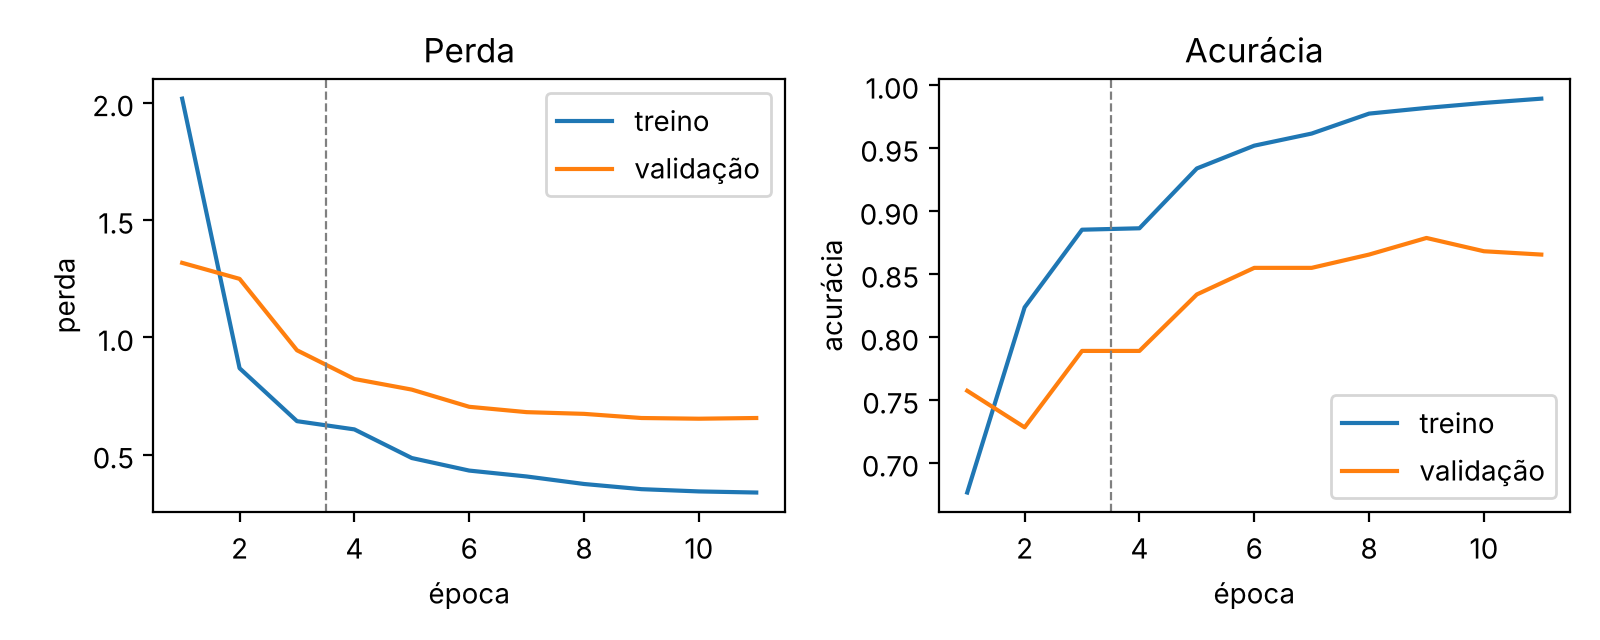
\includegraphics[width=\columnwidth]{../resultados/graficos/curvas_treino.png}
\caption{Perda e acur\'acia por \'epoca. A linha tracejada separa a fase da cabe\c{c}a e o ajuste fino.}
\label{fig:curvas}
\end{figure}

A matriz de confus\~ao (Fig.~\ref{fig:cm}) mostra que as maiores dificuldades est\~ao em ``rejeito'' (F1 de 0,667, com apenas 20 imagens de teste, classe minorit\'aria) e em ``metal'' (precis\~ao de 0,753, pois 9 imagens de pl\'astico, 4 de vidro e 4 de papel foram previstas como metal). A confian\c{c}a m\'edia foi de 0,889 nos acertos e 0,651 nos erros, o que sustenta o uso da confian\c{c}a como crit\'erio de incerteza. Das 48 imagens classificadas incorretamente, 36 tinham confian\c{c}a abaixo de 0,80 e 12 tinham confian\c{c}a igual ou acima de 0,80. Acima de 0,80, a acur\'acia foi de 95,7\% com cobertura de 73,4\% (Fig.~\ref{fig:cov}).

\begin{figure}[t]
\centering
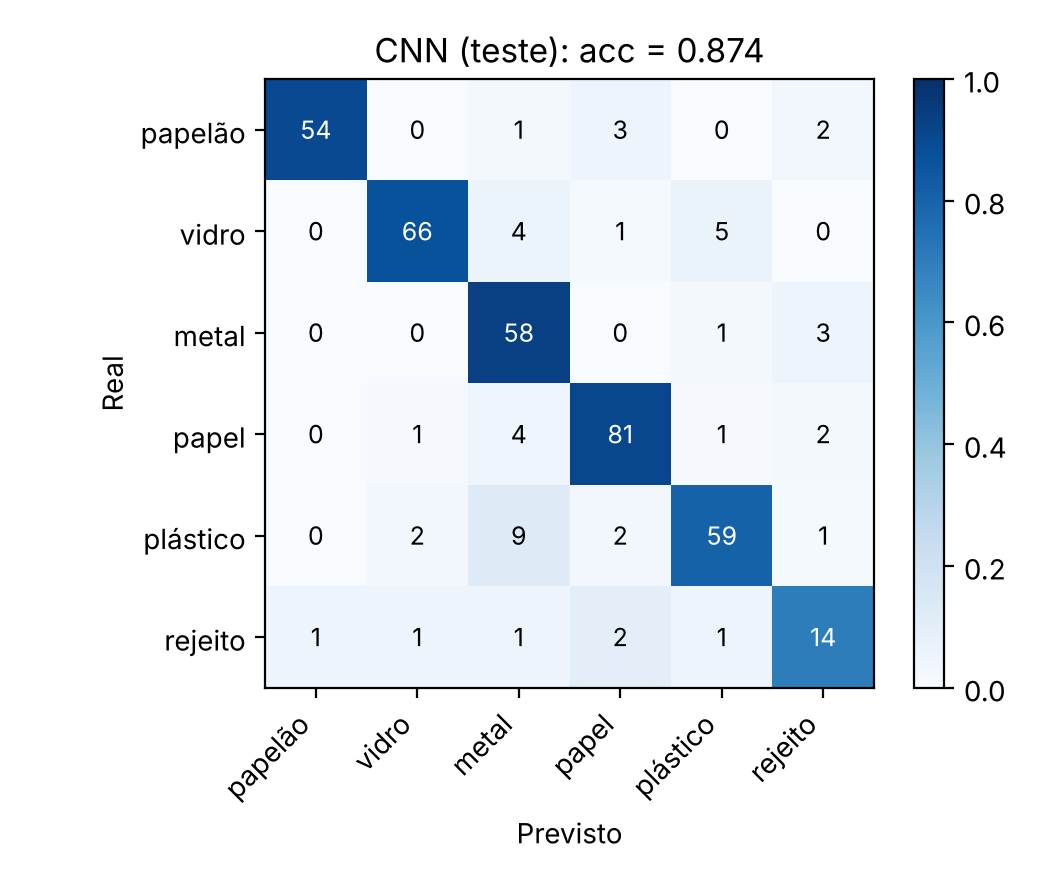
\includegraphics[width=0.85\columnwidth]{../resultados/graficos/matriz_confusao_cnn.png}
\caption{Matriz de confus\~ao da CNN no teste (contagens).}
\label{fig:cm}
\end{figure}

\begin{figure}[t]
\centering
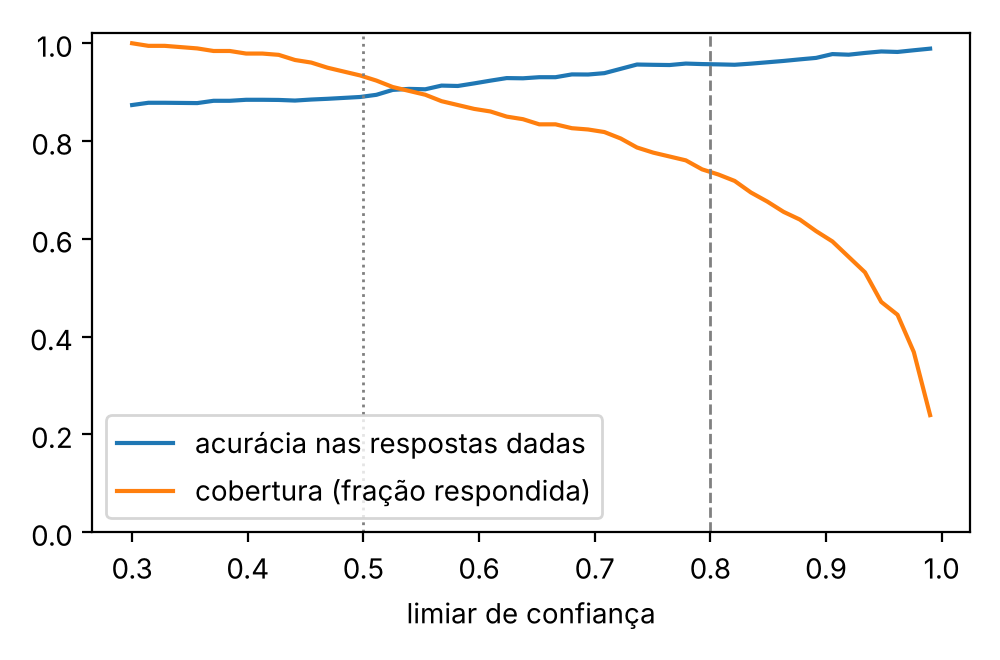
\includegraphics[width=0.95\columnwidth]{../resultados/graficos/cobertura_acuracia.png}
\caption{Acur\'acia nas respostas dadas e cobertura em fun\c{c}\~ao do limiar de confian\c{c}a. Linhas verticais: limiares de 0,50 e 0,80 do agente.}
\label{fig:cov}
\end{figure}

\subsection{PLN}
Na valida\c{c}\~ao cruzada sobre o treino, a Regress\~ao Log\'istica obteve 88,3\% ($\pm$4,9), o LinearSVC 85,8\% ($\pm$5,7) e o Naive Bayes 84,2\% ($\pm$6,7). No corpus de teste de 48 frases in\'editas, o modelo escolhido acertou 45 (93,8\%, F1 macro de 0,937); o Naive Bayes obteve 85,4\%. Os tr\^es erros foram ``de que maneira eu me desfa\c{c}o desse item?'' (previsto como identificar material), ``como preparo isso pra coleta'' (previsto como como descartar) e ``em que local eu deixo isso pra reciclar'' (previsto como pode reciclar), todos com sobreposi\c{c}\~ao lexical com outra inten\c{c}\~ao. Como o corpus \'e pequeno e escrito pela pr\'opria equipe, o valor de 93,8\% tende a ser otimista para perguntas reais.

\subsection{Fluxo integrado e papel do agente}
Para avaliar o fluxo completo, cada imagem de teste foi pareada com uma pergunta sorteada do corpus de teste de PLN (semente fixa). Uma resposta foi considerada correta quando o agente respondeu com o material e a inten\c{c}\~ao corretos. Dos 380 casos, o agente respondeu diretamente em 337, pediu confirma\c{c}\~ao em 9 e pediu nova foto em 34 (8,9\%). Entre os casos em que respondeu, 82,1\% estavam corretos. Para comparar com uma vers\~ao sem o agente (sempre a classe de maior probabilidade e a inten\c{c}\~ao prevista), \'e preciso usar o mesmo denominador: nesses mesmos 346 casos, a vers\~ao sem agente tamb\'em acerta 82,1\%, ou seja, nos casos respondidos o agente n\~ao altera o acerto. Sobre os 380 casos, o acerto sem agente \'e de 80,0\%, contra 74,7\% com o agente: dos 34 pedidos de nova foto, a vers\~ao sem agente teria acertado 20 e errado 14. Portanto, neste conjunto de dados o agente n\~ao melhora a acur\'acia m\'edia; ele evita 14 respostas erradas ao custo de 20 corretas. O valor dele est\'a em comportamentos que essa m\'etrica n\~ao mede: adaptar a orienta\c{c}\~ao \`a condi\c{c}\~ao citada (papel engordurado n\~ao \'e recicl\'avel; vidro quebrado exige embalagem de seguran\c{c}a), arbitrar entre texto e imagem e explicar a decis\~ao. Esses comportamentos s\~ao verificados por testes automatizados no reposit\'orio, mas n\~ao foram avaliados com usu\'arios.

\subsection{Exemplos}
O reposit\'orio inclui exemplos de entrada e sa\'ida (\texttt{resultados/exemplos}), com acertos e erros reais. Em um dos erros, uma caixa de papel\~ao fotografada em \^angulo foi classificada como papel; o agente respondeu normalmente, porque as duas classes s\~ao recicl\'aveis e usam a mesma cor de lixeira, o que reduz o impacto pr\'atico desse tipo de erro.

\subsection{Limita\c{c}\~oes}
(i) O TrashNet tem fundo claro e objeto isolado; o desempenho em fotos do cotidiano, com fundos variados e v\'arios objetos, n\~ao foi medido e tende a ser inferior. (ii) A classe ``rejeito'' tem poucas imagens. (iii) O corpus de PLN \'e pequeno e sint\'etico, e a nega\c{c}\~ao (``n\~ao est\'a limpo'') n\~ao \'e tratada pelo extrator de entidades. (iv) A base de conhecimento segue o c\'odigo de cores do CONAMA e pr\'aticas gerais; regras e pontos de coleta locais precisam ser validados com o \'org\~ao municipal. (v) Os limiares do agente n\~ao foram otimizados conjuntamente. (vi) O agente n\~ao melhorou a acur\'acia m\'edia em rela\c{c}\~ao \`a vers\~ao sem decis\~ao, e seus demais benef\'icios n\~ao foram avaliados com usu\'arios.

\section{Conclus\~ao e Trabalhos Futuros}
O EcoSort demonstrou um fluxo funcional em que vis\~ao, PLN e decis\~ao atuam juntas: a CNN com ajuste fino superou em 15 pontos percentuais um \emph{baseline} cl\'assico (87,4\% contra 72,4\%), o PLN reconheceu 93,8\% das inten\c{c}\~oes inéditas e o fluxo integrado respondeu corretamente 82,1\% dos casos em que respondeu. O agente n\~ao melhorou a acur\'acia m\'edia em rela\c{c}\~ao \`a vers\~ao sem decis\~ao (82,1\% nos mesmos casos respondidos), mas trouxe adapta\c{c}\~ao \`a condi\c{c}\~ao do res\'iduo e explicabilidade. Como trabalhos futuros: treinar com imagens de ambientes reais (por exemplo, TACO) e fotos pr\'oprias, ampliar e diversificar o corpus de perguntas, usar \emph{embeddings} sem\^anticos, tratar nega\c{c}\~ao, calibrar as probabilidades da CNN e cadastrar os pontos de coleta de Macei\'o.

\begin{thebibliography}{99}
\bibitem{yang2016trashnet} M. Yang and G. Thung, ``Classification of Trash for Recyclability Status,'' Stanford CS229 Project Report, 2016. [Online]. Available: \url{https://github.com/garythung/trashnet}
\bibitem{proenca2020taco} P. F. Proen\c{c}a and P. Sim\~oes, ``TACO: Trash Annotations in Context for Litter Detection,'' arXiv:2003.06975, 2020.
\bibitem{deng2009imagenet} J. Deng et al., ``ImageNet: A large-scale hierarchical image database,'' in \emph{Proc. IEEE CVPR}, 2009, pp. 248--255.
\bibitem{howard2019mobilenetv3} A. Howard et al., ``Searching for MobileNetV3,'' in \emph{Proc. IEEE/CVF ICCV}, 2019, pp. 1314--1324.
\bibitem{wightman2019timm} R. Wightman, ``PyTorch Image Models (timm),'' GitHub repository, 2019. [Online]. Available: \url{https://github.com/huggingface/pytorch-image-models}
\bibitem{geifman2017selective} Y. Geifman and R. El-Yaniv, ``Selective classification for deep neural networks,'' in \emph{Advances in Neural Information Processing Systems (NeurIPS)}, 2017.
\bibitem{russell2020aima} S. Russell and P. Norvig, \emph{Artificial Intelligence: A Modern Approach}, 4th ed. Pearson, 2020.
\bibitem{pedregosa2011sklearn} F. Pedregosa et al., ``Scikit-learn: Machine learning in Python,'' \emph{J. Mach. Learn. Res.}, vol. 12, pp. 2825--2830, 2011.
\bibitem{loshchilov2019adamw} I. Loshchilov and F. Hutter, ``Decoupled weight decay regularization,'' in \emph{Proc. ICLR}, 2019.
\bibitem{conama2001} Conselho Nacional do Meio Ambiente (CONAMA), Resolu\c{c}\~ao n$^\circ$ 275, de 25 de abril de 2001: c\'odigo de cores para os diferentes tipos de res\'iduos.
\end{thebibliography}

\end{document}
